\begin{figure}[ht!]
\centering
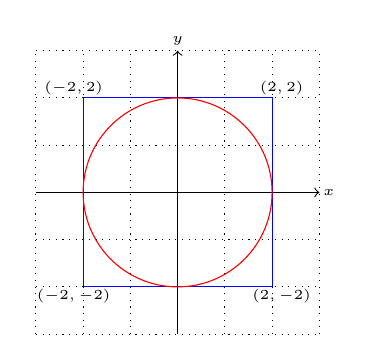
\begin{tikzpicture}[scale=0.6]
% Malla
\draw[thin,dotted] (-3,-3) grid (3,3);
\draw[->] (-3,0) -- (3,0);
% Eje x
\draw (3+.2,0) node {\tiny$x$};
\draw[->] (0,-3) -- (0,3);
% Eje y
\draw (0,3+.2) node {\tiny$y$};
% Cuadrado
\draw[thin, blue] (-2,-2) -- (-2,2) -- (2,2) -- (2,-2) -- cycle;
% Circunferencia
\draw[thin, red] (0,0) circle (2);
\draw (-2-.2,2+.2) node {\tiny$\left(-2,2\right)$};
\draw (2+.2,2+.2) node {\tiny$\left(2,2\right)$};
\draw (-2-.2,-2-.2) node {\tiny$\left(-2,-2\right)$};
\draw (2+.2,-2-.2) node {\tiny$\left(2,-2\right)$};
\end{tikzpicture}
\caption{Circunferencia inscrita en un cuadrado.}
\end{figure}
